\section{Systems Used: Sense2Vec}
The Sense2Vec model is built on a previous method for learning continuous word embeddings known as Word2Vec. Sense2Vec introduces the idea of attaching word senses before beginning the training process this requires part of speech tagging each word in the corpus and is the costliest procedure in the training process. However, the introduction of POS tagging in the process allows a word to be predicted by its surrounding senses rather than by the surrounding words. In base Word2Vec the closest vectors to a supplied word can often be a mixture of proper nouns, verbs and nouns. When supplying the POS with word the query will return a cluster of vectors more relevant to how that word is used. When obtaining the cosine similarity for a proper noun and supplying the POS PROPN Sense2Vec will return vectors more relevant to the use of the noun, this is especially useful when a word can have multiple meanings for example “apple” this could refer to the PROPN of the company Apple or the NOUN apple. Here Sense2Vec is able to extract extra meaning from the word by incorporating the POS of the supplied word, when supplying the word “apple” to Word2Vec the model obtains the cosine similarity of the closest n vectors regardless of where in the sentence the word and the resulting vectors are used. With Sense2Vec a completely different cluster of vectors are obtained when the NOUN and the PROPN are queried resulting in relevant vectors based on the words usage. \cite{Trask2015}

Incorporating POS to obtain extra meaning becomes extremely useful when looking at word depth, as discussed before due to verbs having a much shallower word depth than nouns the meaning of the verb is difficult to extract when using a Word2Vec model. By introducing senses, it allows for the differentiation of a words usage and in turn produces more relevant vectors when using cosine similarity. A comparison of this extra meaning will be shown later in Chapter 4 Results, but one example would be the word “play” with the Word2Vec model there is no differentiation between the verb “to play” and the noun “a play”. Here the resulting n similar vectors would be a combination of both with the verb possibly getting more priority due to more usage than the noun depending on the corpus. Sense2vec removes this ambiguity by differentiating between the verb and the noun which has the result of removing the variable of how often the word is used in each context.

\section{Systems Used: Stanford NLP}
The first step in the training process requires POS tagging each word in the corpus this is the most expensive part of the training process for Sense2Vec. Perfect POS tagging would require constructing a parse tree for the corpus, see Appendix B for further discussion on this process.

However, with the recommendation for Sense2Vec to have a corpus of at least 1 billion words constructing a parse tree of this size for the full corpus would be unfeasible. The Sense2Vec project contains scripts parse and tag a supplied corpus which use the Spacy library made by the same team. This library is relatively new and contains extra features not required for POS tagging, Spacy was not designed as research software and would remove the option for flexibility in the future should it be used. For easier integration and future use of the training methods it was decided that the use of the Stanford NLP library would be used for POS tagging. Stanford NLP has a self-contained python library for which can be used for POS tagging and provides an official Python wrapper for accessing the Java Stanford CoreNLP Server, this allows for the construction of smaller batches of parse trees on segments of the corpus.

This required the rewriting of the original parse process developed by for Sense2Vec using Stanford NLP, once imported the pretrained English models can be downloaded and the pipeline created. This pipeline is what separates Spacy and Stanford, some important options can be configured when using this pipeline. One of which is the Processors option, here it is possible to add or remove processors depending on what is required. In this case the main processor used was the POSPrecessor, however Stanford NLP includes others which provide a more accurately tagged corpus and are required to use the above these include the following:

\begin{itemize}
  \item TokenizeProcessor for segmenting the document into sentences
  \item MWTProcessor for expanding multi-word tokens into multiple words
  \item LemmaProcessor to preform lemmatization of words for example the word "better" has "good" as its lemma.
\end{itemize}
More details on the processors used and the values for each can be found in Appendix E. Each of these processors contain a batch size this is the number of words processed in each batch in this case the default is 5000 and is dependent on the RAM of the computing device. This will be based on the GPU RAM if the use\_gpu is selected when creating the pipeline, in this case a gpu was not used for POS tagging this will be discussed further in the Parsing and POS Tagging section.

\section{Parsing and POS Tagging}
For a fair comparison between Word2Vec and Sense2Vec it was necessary to train both models on the same corpus in this case a corpus of the latest Wikipedia articles was used resulting in a corpus of just over 15GB. This corpus is supplied for public use from Wikipedia and is available online at https://dumps.wikimedia.org/enwiki/ this is a compressed xml file which requires extraction and parsing. The Gensim python library which is used later in training provides a WikiCorpus function for extraction and parsing of each article to text. Each article yields a token where each token was decoded using utf-8 and written to an output file. This wiki.txt output file obtained from WikiCorpusExtractor.py was then used to train both Word2Vec and Sense2Vec models used in Section 3.5 Extracting Results, this process is discussed further in Appendix D.

POS tagging is not required when training Word2Vec however this is what separates the two processes. As discussed earlier Stanford NLP is used when POS tagging the corpus this process is heavily dependent on the RAM of the computing machine and at default the number of words processed during each batch is 5000. With a corpus size of over 15GB it is not possible to load the full corpus into memory for processing as such an iterator is used to return single wiki articles for processing. This assumes the corpus is one document per line and tokens are separated by whitespace. Each line in the corpus is then converted to a doc object for processing by Stanford NLP, once complete the doc object contains sentences which contain words. The .text attribute can be called on this word object to obtain the text and more importantly the .upos attribute contain the universal part of speech tag for the word used in the sentence example NOUN, VERB etc. In cases where the line yielded by the iterator exceeded the memory limit set when creating the Stanford pipeline. The line is broken up into segments less than the size of the word limit and processed as above until the line is complete.

\section{Training}
The process of training for a Word2Vec model is more streamlined than the process for Sense2Vec, once again an iterator is used to obtain single articles from the corpus. This data is passed to the Gensim library containing the Word2Vec, here the min\_count was changed to 1 the training will ignore all words with a frequency less than this value. As discussed in section 2.1 Word2Vec can either use skip gram or CBOW this is decided during training using the sg parameter, in this case both a skip gram and a CBOW model was produced. With Sense2Vec the process of model training is more involved first requiring the input corpus to be POS tagged before any training begins. The bulk of the processing is done using GloVe another project from Stanford NLP. GloVe is designed capture as much as possible the meaning specified by the juxtaposition of two words, take for example “man” and “woman” in one case they can be placed into the category of human however they can also be considered opposites. \cite{Pennington} 

\begin{figure}[h]
    \centering
    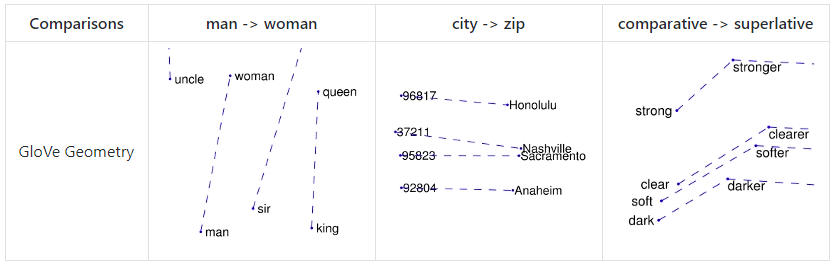
\includegraphics[scale=0.65]{images/GloVe.PNG}
    \caption{Learned Vector Representation}
    \label{fig:GloVe}
\end{figure}

\noindent
Before training can commence three files must be generated using GloVe: 
\begin{itemize}
  \item vocab.txt which stores a list of each unique word in the corpus and its number of occurrences
  \item cooccurrence.bin to store a co-occurrence matrix, which tabulates how frequently words co-occur with one another in the given corpus.
  \item cooccurrence.shuf.bin a shuffled version of the co-occurrence matrix above
\end{itemize}
This process has been completed already by the team behind Sense2Vec and they have supplied the necessary scripts for the GloVe training process. The use of these GloVe and these scripts do come with some caveats and the need for minor edits. GloVe requires the use of bash commands on a Linix system, these commands can however be called from Python itself. The scripts supplied by Sense2Vec use the implementation of f-Strings in Python3.7 in a few cases these commands are formatted incorrectly and require changing. Also of course a major downside to this process is if a Python version less than 3.7 was in use this would require some major changed to the code. Finally, one last script is used 05\_export.py this file loads the vectors file and the frequency file (vocab.txt) and generates a Sense2Vec component that can be loaded via Sense2Vec.from\_disk.

\section{Extracting Results}
Once the models for both Word2vec and Sense2Vec are obtained they can be loaded into memory when needed, both have functions for obtaining n number of cosine similar vectors. While it is a straightforward process to query the models one other benchmark is used against the two systems, WordNet allows the use of a path similarity value between two synsets. This process is somewhat cumbersome as the path similarity method must be called on one synset object passing the comparison synset object as an argument. As such a small wordnet\_similarity function was created to compare path similarity between two words. One major advantage of this is that WordNet itself contains POS tags for each synset and so a benchmark can be used against Sense2Vecs use of POS tagging.

Some of the results are used to highlight Sense2Vecs ability over Word2Vec and WordNet however as to avoid cherry picking results some randomness and statistical methods are used. The first of these methods involves two large noun and verb text files. By obtaining 1000 random words from each a query is performed on WordNet using the random word. The synsets for this word are obtained from Wordnet with the first word from the first synset, the last word from the first synset and the last word from the last synset being returned. A comparison is then made between the similarities of each of the three words using both Word2Vec and Sense2Vec. Another form of verification is also introduced using Bloom’s taxonomy which is used to classify educational learning objectives into levels of complexity. Each of these levels contain verbs the describe the action at each level, the similarity is calculated between each verb in each level using both Word2Vec and Sense2Vec. With both of the methods above statistical analysis is preformed through the use of the R language, in the case of Bloom’s taxonomy each level receives its own boxplot containing the similarity scores.